
\documentclass[a4paper, 10pt]{IEEEconf}  

\usepackage{geometry}
\geometry{a4paper, margin=1in}
  
  
\usepackage{subcaption}  
\usepackage[export]{adjustbox}    
\usepackage{verbatim}
\usepackage{graphicx}
\usepackage{pdfpages}
\usepackage{cite}
\usepackage{listings}
\usepackage{float}
\usepackage{url}
\usepackage{hyperref}
\usepackage{fancyhdr}
\usepackage{multicol}

\lstset{
	tabsize=2,
	breaklines=true
}

\setlength{\parskip}{1em}
\onecolumn

\title{\LARGE \bf Assignment 3: TensorFlow Neural Network Training\\Industrial Systems Design and Integration 282 772}
\author{Marc Alexander Sferrazza \\ 12164165
\thanks{This work was not supported by any organization}
\thanks{Faculty of Mechatronics Engineering, Massey University, Albany, Auckland, New Zealand
        {\tt\small Progress of project: https://github.com/alex1v1a/Industrial-Systems-Design-and-Integration} } }

\begin{document}

\maketitle
%\begin{figure}[h]
%\begin{subfigure}{0.5\textwidth}
%\includegraphics[width=1.5\textwidth, left]{images/ROS} 
%%\caption{ROS}
%\label{fig:ROS}
%\end{subfigure}
%\begin{subfigure}{0.5\textwidth}
%\includegraphics[width=0.3\textwidth, right]{images/gazebo}
%%\caption{Gazebo} 
%\label{fig:Gazebo}
%\end{subfigure}
%%\caption{Caption for this figure with two images}
%%\label{fig:image2}
%\end{figure}
\begin{figure}[H]
  \begin{center}
  
\includegraphics[width=110mm]{images/tf}
  \label{fig:kinetic}
  \end{center}
\end{figure}
\thispagestyle{empty}
\pagestyle{plain}


%%%%%%%%%%%%%%%%%%%%%%%%%%%%%%%%%%%%%%%%%%%%%%%%%%%%%%%%%%%%%%%%%%%%%%%%%%%%%%%%

\begin{abstract}
In this documentation TensorFlow's neural network machine learning is used to find a function for y=f(x) given some inputs and outputs. The process involves using the Multi-Layered Perceptron (MLP) technique training and placeholders are used to provide input.
\end{abstract}


\clearpage
\thispagestyle{empty}
\tableofcontents
\begingroup
\let\clearpage\relax
\listoffigures
%\listoftables
\endgroup
%\thispagestyle{empty}
\clearpage
\twocolumn

%%%%%%%%%%%%%%%%%%%%%%%%%%%%%%%%%%%%%%%%%%%%%%%%%%%%%%%%%%%%%%%%%%%%%%%%%%%%%%%%
%%%%%%%%%%%%%%%%%%%%%%%%%%%%%%%%%%%%%%%%%%%%%%%%%%%%%%%%%%%%%%%%%%%%%%%%%%%%%%%%
\clearpage
\setcounter{page}{1}
%\thispagestyle{empty}
\onecolumn

\section{INTRODUCTION}

TensorFlow is a free python language based library which is used for machine learning using neural networks to determine functions based on given inputs and outputs. As TensorFlow (TF) is supported by the community it makes as a favourable tool to learn, and is not only capable of black box systems, but also able to coordinate with complex systems with learning nodes.

In this documentation the program TensorFlow is used to train a neural network that will approximate an unknown function of y=f(x) for a given vector. Using Python 3.5+ syntax and TensorFlow 1.0+ syntax, a predefined data set csv file will be called on which to preform the learning task for an output range.


%%%%%%%%%%%%%%%%%%%%%%%%%%%%%%%%%%%%%%%%%%%%%%%%%%%%%%%%%%%%%%%%%%%%%%%%%%%%%%%%

\subsection{Installation}

As TensorFlow uses Python, it supports multiple platforms including Mac, Windows, Linux, and Chrome OS. I have successfully installed Python 3.6 with a TensorFlow Python 3.5 CPU based workspace from source and have things compiled nicely; however for consistency with the lectures at Massey and to avoid any unnecessary errors I have completed these tasks using the advised programs with Visual Studio's CODE on Windows 10 OS. To setup and install TensorFlow simply follow the instructions on the TensorFlow website, or see the Getting Started with TensorFlow video on Frazer Nobles YouTube channel \cite{tfinstall}

When setting up TensorFlow it features to automatically add to the environmental variables PATH, however the Python version and must be set to 3.5 manually (due to current version of 3.6), along with the option for CPU or GPU compiling. Visual Studios CODE is installed as the editor with a built in terminal cmd for quick compiling. Finally after setting up and installing TensorFlow with Python and CODE, a test program is written to check the status of the install with success.

\begin{figure}[H]
  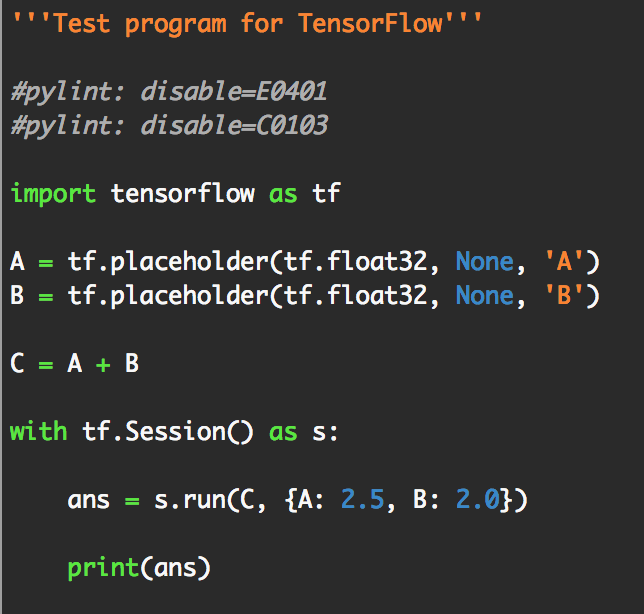
\includegraphics[width=0.5\linewidth, center]{images/test}
  \caption{Test file to check the working status for TensorFlow install, Result = 4.5}
  \label{fig:Test file to check the working status for TensorFlow install, Result = 4.5}
\end{figure}

%%%%%%%%%%%%%%%%%%%%%%%%%%%%%%%%%%%%%%%%%%%%%%%%%%%%%%%%%%%%%%%%%%%%%%%%%%%%%%%%
%%%%%%%%%%%%%%%%%%%%%%%%%%%%%%%%%%%%%%%%%%%%%%%%%%%%%%%%%%%%%%%%%%%%%%%%%%%%%%%%
%\clearpage
\section{METHOD}

Using TensorFlows neural network training MLP method, an approximation can be made for the y=f(x) function. As discussed in the lectures to revise what was mentioned, the training method involves the input to segment blocks, where it is compared and examined with the relationship of output in a set shape space. The learning rate is the increment of which will define how well the relationship can be made with the smoothest function; this over iterations with a certain node size (mutations) and can give a higher accuracy with more reliable results of many iterations. 

%%%%%%%%%%%%%%%%%%%%%%%%%%%%%%%%%%%%%%%%%%%%%%%%%%%%%%%%%%%%%%%%%%%%%%%%%%%%%%%%

\subsection{Multi-Layered Perceptron (MLP) Training}

Multi-Layered Perceptron (MLP) is used..... and trained

Placeholders are used to provide input


Using this training method ....


%%%%%%%%%%%%%%%%%%%%%%%%%%%%%%%%%%%%%%%%%%%%%%%%%%%%%%%%%%%%%%%%%%%%%%%%%%%%%%%%
%\clearpage
\subsection{Importing the CSV}

A csv file, containing pairs of x and y values is read into the .....




%2. Add a screenshot of ROSCORE running in a terminal 
%Roscore is the fundamental processing command on which ROS can activate the simulation environment; from here gazebo can spawn models which can be edited with plugins and controlled via nodes as explained later.
%
%\begin{figure}[H]
%\begin{subfigure}{\textwidth}
%	\begin{center}
%  	\includegraphics[width=0.7\textwidth]{images/ROSCORE}
%  	\label{fig:ROSCORE running in terminal Mac Desktop}
%  	\end{center}
%\end{subfigure}
%\begin{subfigure}{\textwidth}
%	\begin{center}
%  	\includegraphics[width=0.7\textwidth]{images/ROSCORE2}
%  	\label{fig:ROSCORE running in terminal enlarged}
%  	\end{center}
%\end{subfigure}
%\end{figure}
%
%Above is a demonstration of ROSCORE running in a terminal on Ubuntu operating system. This is currently in coherent mode but for better performance in later tasks the virtual runtime is switched to windowed mode.

%%%%%%%%%%%%%%%%%%%%%%%%%%%%%%%%%%%%%%%%%%%%%%%%%%%%%%%%%%%%%%%%%%%%%%%%%%%%%%%%
%\clearpage
\subsection{Nodes}

when you have a slow learning rate, you need more iterations, 

but if you have a higher learning rate you waste alot of time getting stuck in local minimuns

lower learning rate, learns more finely...

The more node you have the more variations you have

The more different types of variations it will try

If you have 3 nodes you have 

source code can be adapted to plot the given x and y values and the neural network's inferred output

%5. What links the simulated robot in Gazebo to ROS nodes? A good explanation with figures and/or codes snippets is required.
%Using some of the default plugins provided from the ROS package site, in this case the "Differential Drive" we can assign the left and right joints (wheels) to the controller. The controller in turn will take the response value passed from the Teleop Node and preform the movement in the joint.
%
%\begin{figure}[H]
%\begin{subfigure}{\textwidth}
%	\begin{center}
%  	\includegraphics[width=0.7\textwidth]{images/Plugin}
%  	\label{fig:Using plugins provided from ROS}
%  	\end{center}
%\end{subfigure}
%\begin{subfigure}{\textwidth}
%	\begin{center}
%  	\includegraphics[width=0.7\textwidth]{images/Plugin2}
%  	\label{fig:Applying the plugin}
%  	\end{center}
%\end{subfigure}
%\end{figure}
%
%Note: The highlighted text is copied directly without the "gazebo" tags; also once the plugin is added to the model sdf file it is then edited with gedit to match the joint name values e.g. left wheel and so on.
%
%\clearpage
%Again we can do this for the laser plugin and add the plugin to the create model 1.4
%
%\begin{figure}[H]
%  \includegraphics[width=0.8\linewidth, center]{images/laser}
%  \caption{laser plugin node setup}
%  \label{fig:laser plugin node setup}
%\end{figure}
%
%Here is the model with the laser scanner attached
%
%\begin{figure}[H]
%  \includegraphics[width=0.8\linewidth, center]{images/laserdemo}
%  \caption{laser plugin node mesh graphic}
%  \label{fig:laser plugin node mesh graphic}
%\end{figure}
%
%After the plugin is assigned to the sdk file the subscriber nodes can be setup. By creating a package and compiling it, the executables can then be run and useful output given from various broadcasted topics.
%
%\clearpage
%Below is a demonstration of the odometry topic, and a node being used to give the user a notice when the 5 meter mark has bene reached in along the x and y axis. 
%
%\begin{figure}[H]
%  \includegraphics[width=0.8\linewidth, center]{images/odomcode}
%  \caption{Subscriber odom node setup}
%  \label{fig:Subscriber odom node setup}
%\end{figure}
%
%Here is the cpp code for the subscriber to the cmd velocity topic.
%
%\begin{figure}[H]
%  \includegraphics[width=0.8\linewidth, center]{images/cmdvelcode}
%  \caption{Subscriber cmd vel node setup}
%  \label{fig:Subscriber cmd vel node setup}
%\end{figure}
%
%\clearpage
%Then the new cpp files are added to the cmake file to be compiled as executables the next time catkin make command is called.
%
%\begin{figure}[H]
%  \includegraphics[width=0.8\linewidth, center]{images/exe}
%  \caption{nodes executables setup}
%  \label{fig:nodes executables setup}
%\end{figure}
%
%After completing and running the new node when the subscriber receives information from the broadcaster; it is then displayed on the console like the following.
%
%\begin{figure}[H]
%  \includegraphics[width=0.8\linewidth, center]{images/cmdvelsub}
%  \caption{A demo showing the cmd vel node being executed, output from the moving model}
%  \label{fig:A demo showing the cmd vel node being executed, output from the moving model}
%\end{figure}


%%%%%%%%%%%%%%%%%%%%%%%%%%%%%%%%%%%%%%%%%%%%%%%%%%%%%%%%%%%%%%%%%%%%%%%%%%%%%%%%
%\clearpage
\subsection{Base Optimizer}



%4. Include screenshots of "teleop node" and the robot in Gazebo at different positions. This should not be more than one page. 
%Below is a demonstration of the Teleop Node used to control the left and right wheels with the plugins mentioned earlier.
%
%\begin{figure}[H]
%\begin{subfigure}{\textwidth}
%	\begin{center}
%  	\includegraphics[width=0.7\textwidth]{images/Teleop}
%  	\label{fig:Teleop node running on ubuntu}
%  	\end{center}
%\end{subfigure}
%\begin{subfigure}{\textwidth}
%	\begin{center}
%  	\includegraphics[width=\textwidth]{images/Position}
%  	\label{fig:A model iRobot Create spawned in Gazebo using teleop node for movements}
%  	\end{center}
%\end{subfigure}
%\end{figure}
%
%Shown above is the rviz graphical representation of the odometry, the purple vertical lines represent the position while the red arrows show the directional vector. Rviz is great for graphical demos of what the robot interacts with in the model environment, e.g a scanner attached to find a obstacles and other objects.
%
%\clearpage
%Again Shown the rviz using the laser node with obstruction blocks and the subscribed laser topic, the representation is given by flat squares in red.
%
%\begin{figure}[H]
%  \includegraphics[width=0.8\linewidth, center]{images/rvizlaser}
%  \caption{A demo showing the cmd vel node being executed, output from the moving model}
%  \label{fig:A demo showing the cmd vel node being executed, output from the moving model}
%\end{figure}

%%%%%%%%%%%%%%%%%%%%%%%%%%%%%%%%%%%%%%%%%%%%%%%%%%%%%%%%%%%%%%%%%%%%%%%%%%%%%%%%
%%%%%%%%%%%%%%%%%%%%%%%%%%%%%%%%%%%%%%%%%%%%%%%%%%%%%%%%%%%%%%%%%%%%%%%%%%%%%%%%

\section{RESULTS}

Original Data set \& Inferred Output is shown 

An image illustrating the original data set and the inferred output of your program.

After successfully configuring the Multi-Layered Perceptron (MLP), reading in the values in the provided csv

\begin{figure}[H]
  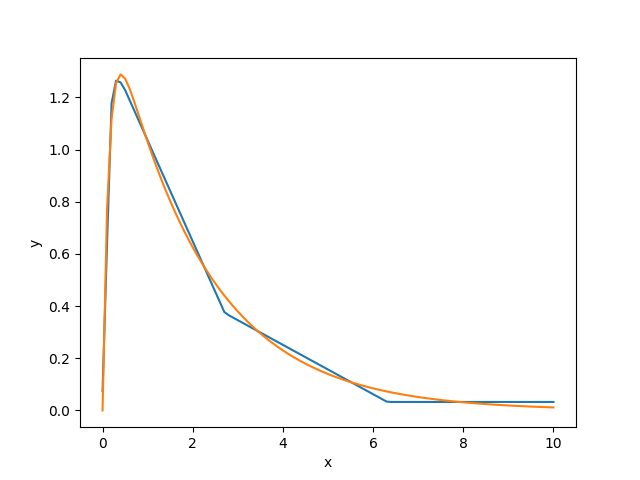
\includegraphics[width=0.8\linewidth, center]{images/plot}
  \caption{The final resultant is shown in compare on a graph}
  \label{fig:The final resultant is shown in compare on a graph}
\end{figure}

Once the initial results were found, to further the accuracy of the output the training of the MLP using the Adam Optimiser algorithum was used as suggested in class, please see variable for assigned learn rate in the code in the appendix. Below is the revised version using the Adam optimiser with specified nodes and learning rates as described in the logic documentation \cite{adam}. A clear difference between the optimiser reflects the accuracy for the learning of the function in this case.

\begin{figure}[H]
  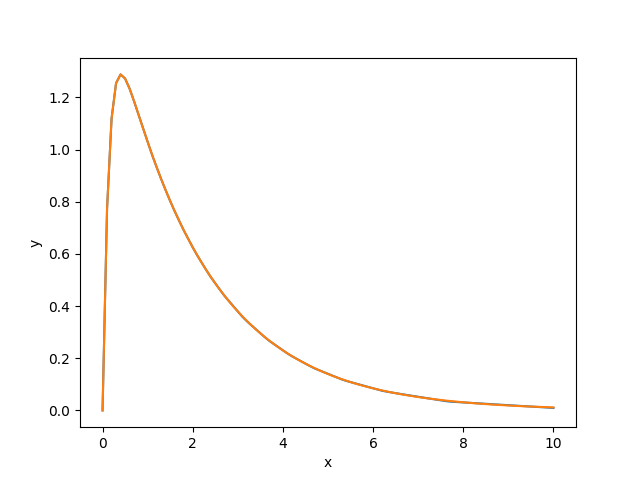
\includegraphics[width=0.8\linewidth, center]{images/3}
  \caption{The final resultant is shown in compare on a graph}
  \label{fig:The final resultant is shown in compare on a graph}
\end{figure}

%%%%%%%%%%%%%%%%%%%%%%%%%%%%%%%%%%%%%%%%%%%%%%%%%%%%%%%%%%%%%%%%%%%%%%%%%%%%%%%%
%%%%%%%%%%%%%%%%%%%%%%%%%%%%%%%%%%%%%%%%%%%%%%%%%%%%%%%%%%%%%%%%%%%%%%%%%%%%%%%%

\section{OUTCOMES}

%Through the above steps ROS has been successfully installed, the Gazebo runtime is used with the catkin workspace to spawn a model with edited plugins that are able to be controlled via the teleop node. 
%
%The output is then displayed on the rviz graphical demonstration. A custom node is implemented to subscribe to the velocity topic and display the variable speed with a mentioned warning.


%%%%%%%%%%%%%%%%%%%%%%%%%%%%%%%%%%%%%%%%%%%%%%%%%%%%%%%%%%%%%%%%%%%%%%%%%%%%%%%%
%%%%%%%%%%%%%%%%%%%%%%%%%%%%%%%%%%%%%%%%%%%%%%%%%%%%%%%%%%%%%%%%%%%%%%%%%%%%%%%%

\section{CONCLUSIONS}

For any progress related to the report please see the public Github repo for alex1v1a or use the link in the cover page to be automatically redirected to this project. The repo provides all relative project information

I have come to a further understanding learned the fundamentals of TensorFlow with the use of such machine learning tools like Multi-Layered Perceptron using placeholders. This is a powerful tool and from the basic level of understanding is an strong aspect of the machine learning processing, it is a great skill to learn.

%%%%%%%%%%%%%%%%%%%%%%%%%%%%%%%%%%%%%%%%%%%%%%%%%%%%%%%%%%%%%%%%%%%%%%%%%%%%%%%%
%%%%%%%%%%%%%%%%%%%%%%%%%%%%%%%%%%%%%%%%%%%%%%%%%%%%%%%%%%%%%%%%%%%%%%%%%%%%%%%%

\nocite{*}
\bibliographystyle{ieeetr}
\bibliography{references}

%%%%%%%%%%%%%%%%%%%%%%%%%%%%%%%%%%%%%%%%%%%%%%%%%%%%%%%%%%%%%%%%%%%%%%%%%%%%%%%%
%%%%%%%%%%%%%%%%%%%%%%%%%%%%%%%%%%%%%%%%%%%%%%%%%%%%%%%%%%%%%%%%%%%%%%%%%%%%%%%%

\clearpage
\onecolumn
\section*{APPENDIX}
\begin{lstlisting}[language = Python]
# pylint: disable=C0413
# pylint: disable=C0103
# pylint: disable=E0401

import os
import tensorflow as tf # TesnorFlow Librarys
import csv # For csv importing etc
import matplotlib.pyplot as plt # For graphing and plotting etc

# Adjustable Values, Nodes, Learning Rate, and epochy 
nodeSize = 300 # More variation, more mutation
learnRate = 0.005 # Lower the learning rate the higher accuracy
iteration = 300000 # How many times it wil go through - epochy

os.environ['TF_CPP_MIN_LOG_LEVEL'] = '3' # Suppresses warnings

# Import csv file, assign coloums as inputX, inputY respectivly, no determined allocation size for memory
inputX = [] 
inputY = [] 
# Open and read in data_set.csv
with open('data_set.csv','r') as csvfile: 
    plots = csv.reader(csvfile, delimiter=',') 
    for row in plots: 
		# Add each line of the csv to the row array for X and Y
        inputX.append([float(row[0])]) 
        inputY.append([float(row[1])])

# Placeholders are used, tensorflow diag 32 type with shape of nil, 1 - labeled x and y respectivly
x = tf.placeholder(dtype=tf.float32, shape=[None, 1], name='x')
y = tf.placeholder(dtype=tf.float32, shape=[None, 1], name='y')

# MLP
def mlp_layer(in_x, w_shape, b_shape):
    '''mlp_layer'''
	# Using the get variable function with the passed through same shapes and random initializer with no conditions
    W = tf.get_variable(name='W', shape=w_shape, dtype=tf.float32,
                        initializer=tf.random_uniform_initializer())
    b = tf.get_variable(name='b', shape=b_shape, dtype=tf.float32,
                        initializer=tf.random_uniform_initializer())
	# Assign the output of the added variables with shape b					
    out_y = tf.add(tf.matmul(in_x, W), b)
	# Return the addition of the layer as passthrough
    return out_y

# Layer 1 computation
with tf.variable_scope('layer_1') as vs:
    h = mlp_layer(x, [1, nodeSize], [nodeSize])
    h = tf.nn.relu(h)
    vs.reuse_variables()

# Layer 2 computation
with tf.variable_scope('layer_2') as vs:
    y_ = mlp_layer(h, [nodeSize, 1], [1])

# Loss value for the mean squared error
loss = tf.losses.mean_squared_error(y, y_)
# Training of the MLP using the Adam Optimizer as suggested in class, please see variaible for assigned learn rate
training = tf.train.AdamOptimizer(learning_rate=learnRate).minimize(loss)

# We must initalize the tensorflow with both global and local
init = [tf.global_variables_initializer(), tf.local_variables_initializer()]

# Begin the learing session after everything is setup and imported
with tf.Session() as s:
	# Run the initializer for the session
    s.run(init)

	# After evaluating the shape, this section was removed and shaped on the import of the csv
    # x1 = s.run(tf.reshape(inputX, [101,1])) 
    # y2 = s.run(tf.reshape(inputY, [101,1]))

	# Begin the loop for the function of the assigned iteration steps.
    for i in range(0, iteration, 1):
		# Start the training 
        l, _ = s.run([loss, training], feed_dict={x: inputX, y: inputY})

		# Only print the 10 cycles of iterations - epochy ~ 1st Jan 1970 lol...
        if i % (iteration/10) == 0:
			# Print the trained value..
            print(l)
	
	# Assign the learning points to use for the plot
    p = s.run(y_, {x:inputX}) 
	# Plot the learning points
    plt.plot(inputX,p) 
	# Plot the origional csv values
    plt.plot(inputX, inputY) 
	# Label Axis etc...
    plt.xlabel('x') 
    plt.ylabel('y') 
	# Show plot
    plt.show()
\end{lstlisting}

\end{document}
